\documentclass{beamer}

\usepackage[utf8]{inputenc}
\usepackage[T1]{fontenc}
\usepackage{textpos}
\usepackage{tikz}

\usetheme{Madrid}
\usecolortheme{beaver}

% Custom changes:
\setbeamertemplate{footline}[frame number]{}
\definecolor{university_tuebingen}{RGB}{165,30,55}
\setbeamercolor{frametitle}{fg=university_tuebingen, bg=white}
\setbeamercolor{title}{fg=university_tuebingen}

\addtobeamertemplate{frametitle}{}{
\begin{tikzpicture}[remember picture, overlay]
\node[anchor=north east,yshift=0cm] at (current page.north east)
{
\includegraphics[width=3cm]{../common/logo_uni_tuebingen2.png}};
\end{tikzpicture}}



\author{Prof. Dr. Christiane Zarfl, Dipl.-Inf. Willi Kappler}
%\date{\today}
\date{}
%\institute{Universität Tübingen}
\institute{}


\matlabTitle{1. Grundlagen}

% Rechtschreibprüfung mit: aspell -l de -t --tex-check-comments -c lecture1/lecture1.tex

\setcounter{mchapter}{1}
\setcounter{mexercise}{0}

\begin{document}
    {
\beamertemplatenavigationsymbolsempty % suppress navigation on this (= first) slide
\begin{frame}[plain] % plain means: no header and footer on this (= first) slide
    \begin{textblock*}{0cm}(0.5cm, -0.7cm)
        
\includegraphics[width=11.0cm]{../common/logo_uni_tuebingen.png}
    \end{textblock*}
    \titlepage
    \begin{textblock*}{0cm}(0.1cm, -2.5cm)
        \textcolor{university_tuebingen}{\rule{11.8cm}{0.2cm}}
    \end{textblock*}
\end{frame}
}


    \section{Einleitung}

    \subsection{Konventionen}
    \begin{frame}
        \frametitle{Verwendete Konventionen 1}
        \begin{itemize}
            \item In diesen Kursunterlagen werden die folgenden Konventionen verwendet:
            \item Eingabetext wird grün hinterlegt, z.B.: \matlabInput{plot}
            \item Alle Ausgaben werden blau hinterlegt, z.B.: \matlabOutput{a = 12.78}
            \item Beispielprogramme werden grün hinterlegt mit Zeilennummern abgebildet und die Ausgabe dieser Programme
            wird blau hinterlegt, z.B.:
        \end{itemize}
        \vspace{-0.5cm}
        \insertMatlabCodeOutput{example1_0}
    \end{frame}

    \begin{frame}
        \frametitle{Verwendete Konventionen 2}
        \begin{itemize}
            \item Hyperlinks auf Webseiten werden mit blauem Text gekennzeichnet, \\
            z.B.: \urlLink{http://www.uni-tuebingen.de}{Uni Tübingen - klick mich}
            \item Menüeinträge werden durch hellgraue Kästen dargestellt, \\
            z.B.: \menu{Datei > Speichern}
            \item Datei- / Verzeichnispfade werden durch kleine Pfeile symbolisiert: \directory{Eigene Dateien / Matlab / Uebung1}
            \item Tastenkürzel (Shortcuts) und Eingaben werden ebenfalls in hellgrauen Kästen dargestellt, z.B.: \keys{F10}, \keys{\return}, \keys{\ctrl+a}
            \item Übungsaufgaben werden in einem gelben Kasten abgebildet, z.B.:
        \end{itemize}
        \begin{exercise}
            \sloppy
            Übung 1: Berechnen Sie die ersten 20 Dezimalziffern der Zahl $\pi$.
        \end{exercise}
    \end{frame}

    \subsection{Warum Matlab ?}
    \begin{frame}
      \frametitle{Matlab - Warum ?}
      \begin{textblock*}{0cm}(5.0cm, -1.0cm)
        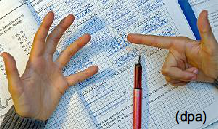
\includegraphics[width=3.0cm]{rechnen1.png}
      \end{textblock*}
      \begin{textblock*}{0cm}(9.0cm, 0.0cm)
        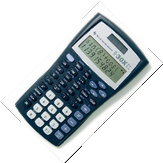
\includegraphics[width=2.0cm]{rechnen2.png}
      \end{textblock*}

      \begin{itemize}
        \itemsep0.4cm
        \item Einfache Rechnungen
        \item Datenaufbereitung \& -speicherung
        \item Visualisierung von Daten \& Simulationsergebnissen
        \item einfaches Lösen von (linearen) Gleichungssystemen, Differentialgleichungen (DGL), DGL-Systemen...
        \item Wiederverwendung von häufig gebrauchten Berechnungen (Programmierung)
        \item Datenanalyse (z.B. Regression) \& Statistik
        \item Komplexe Modellierung von Umweltsystemen
      \end{itemize}
    \end{frame}

    \subsection{Visualisierung}
    \begin{frame}
      \frametitle{Matlab - Warum ?}
      \vspace{-0.8cm}
      \begin{figure}
        Visualisierung von Daten \& Simulationsergebnissen \par \vspace{0.4cm}
        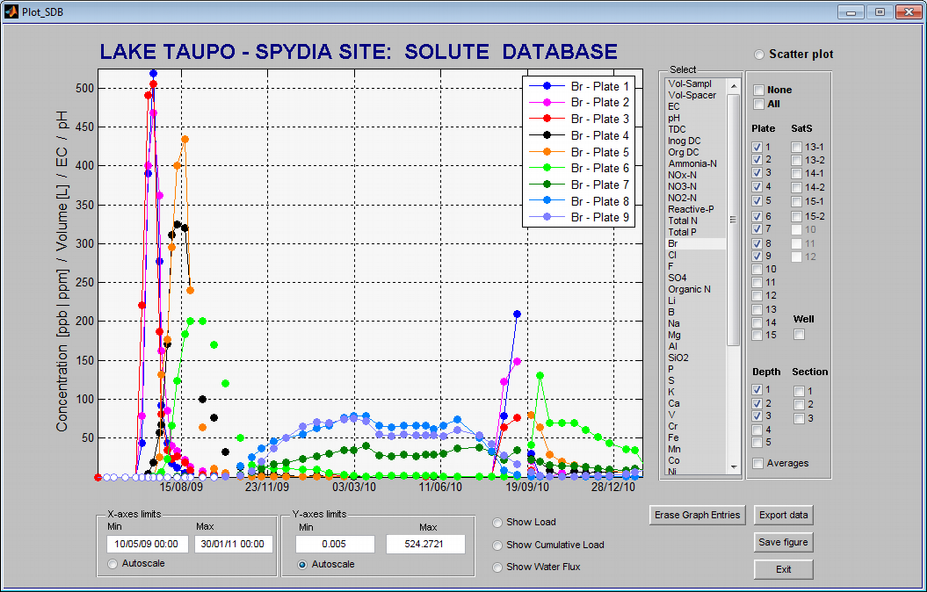
\includegraphics[width=10.0cm]{visualisierung1.png}
      \end{figure}
    \end{frame}

    \subsection{Datenalalyse}
    \begin{frame}
      \frametitle{Matlab - Warum ?}

      \vspace{-0.8cm}

      \begin{figure}
        Datenanalyse \& Statistik \par \vspace{0.4cm}
        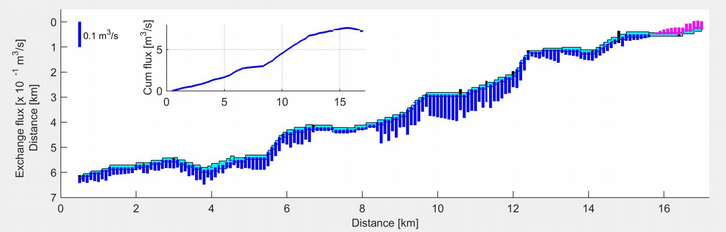
\includegraphics[width=10.0cm]{visualisierung2.png}
      \end{figure}

      \vspace{-0.5cm}

      \begin{figure}
        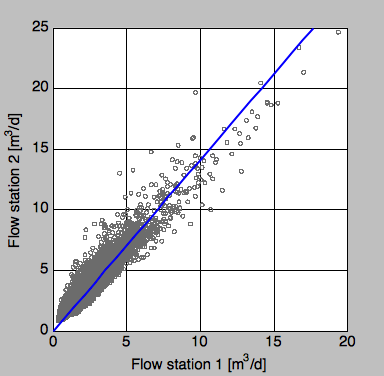
\includegraphics[width=3.0cm]{visualisierung3.png}
        \hspace{0.5cm}
        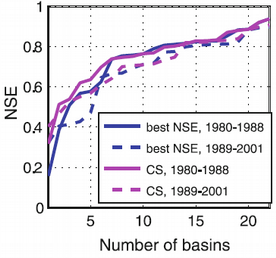
\includegraphics[width=3.0cm]{visualisierung5.png}
        \hspace{0.5cm}
        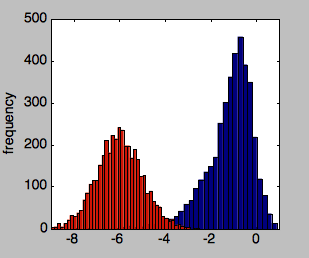
\includegraphics[width=3.0cm]{visualisierung4.png}
      \end{figure}
    \end{frame}

    \subsection{Modellierung}
    \begin{frame}
      \frametitle{Matlab - Warum ?}
      \vspace{-0.8cm}
      \begin{figure}
        Modellierung von Umwelstsystemen \par \vspace{0.4cm}
        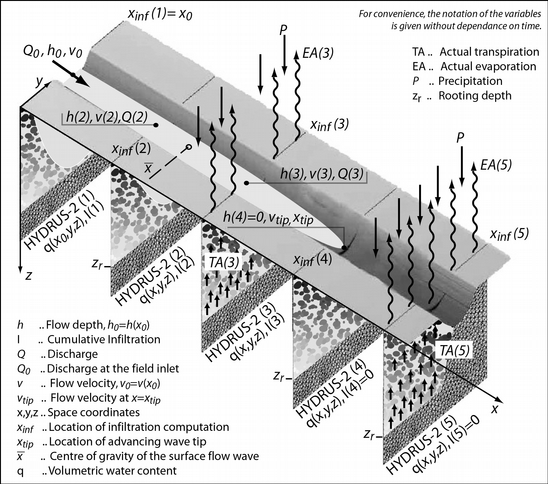
\includegraphics[width=7.5cm]{modellierung1.png}
      \end{figure}
    \end{frame}

    \subsection{Organisatorisches}
    \begin{frame}
        \frametitle{Organisatorisches}

        \vspace{-1.0cm}

        \begin{itemize}
          \item Hardware:

          \begin{itemize}
            \itemsep0.3cm
            \item BYOD (eigenes Gerät mitbringen)
            \item Geo-Notebooks (Raum S245)
            \item CIP Pool Rechner (Raum S310)
          \end{itemize}

          \item Software:

          \begin{itemize}
            \itemsep0.3cm
            \item Auf Institutshardware bereits vorinstalliert
            \item ZDV: Matlab \urlLink{https://services.zdv.uni-tuebingen.de/CampusSoftware/}{herunterladen}
            \item \urlLink{https://www.gnu.org/software/octave/}{GNU Octave } (Open Source, aber nicht 100\% kompatibel)
          \end{itemize}

          \item \alert{Auf Institutshardware bitte zuerst ein eigenes Verzeichnis anlegen!}

        \end{itemize}
    \end{frame}

    \subsection{Was ist Matlab}
    \begin{frame}
        \frametitle{Was ist Matlab}
        \begin{itemize}
          \item ``\emph{Matlab} ist eine kommerzielle Software des Unternehmens \emph{The MathWorks, Inc.} zur Lösung mathematischer Probleme
          und zur grafischen Darstellung der Ergebnisse.'' (Quelle: \urlLink{https://de.wikipedia.org/wiki/Matlab}{Wikipedia}).
          \item Matlab leitet sich ab von \textbf{MAT}rix \textbf{LAB}oratory.
          \item Wir benutzen Matlab als (nummerische) Programmiersprache.
          \item Wie ein Taschenrechner oder Excel arbeitet Matlab nummerisch (mit Zahlenwerten, also nicht symbolisch wie
          ein \urlLink{https://de.wikipedia.org/wiki/Computeralgebrasystem}{CAS}).
          \item Anders als bei einem Taschenrechner können Zahlenwerten Variablennamen zugewiesen werden.
          \item Im Programm werden die Variablennamen als Platzhalter für die Werte verwendet.
        \end{itemize}
    \end{frame}

    \subsection{Motivation}
    \begin{frame}
        \frametitle{Nach dieser ersten Kurseinheit...}
        \begin{itemize}
          \itemsep0.3cm
          \item kennen Sie den Aufbau der Oberfläche der Software Matlab.
          \item benutzen Sie die Matlab-Hilfe, um für Sie nützliche Funktionen und Informationen selbstständig zu finden.
          \item führen Sie einfache Rechnungen mit Matlab durch.
          \item können Sie Variablen in Matlab definieren und verwenden.
          \item kennen Sie die Vorteile der Verwendung von Vektoren und können diese in Matlab definieren und für Rechnungen verwenden.
        \end{itemize}
    \end{frame}

    \subsection{GUI}
    \begin{frame}
      \frametitle{Die Matlab GUI}

      \vspace{-0.8cm}

      \begin{figure}
        \begin{tikzpicture}
          \node[anchor=south west,inner sep=0] (image) at (0,0) {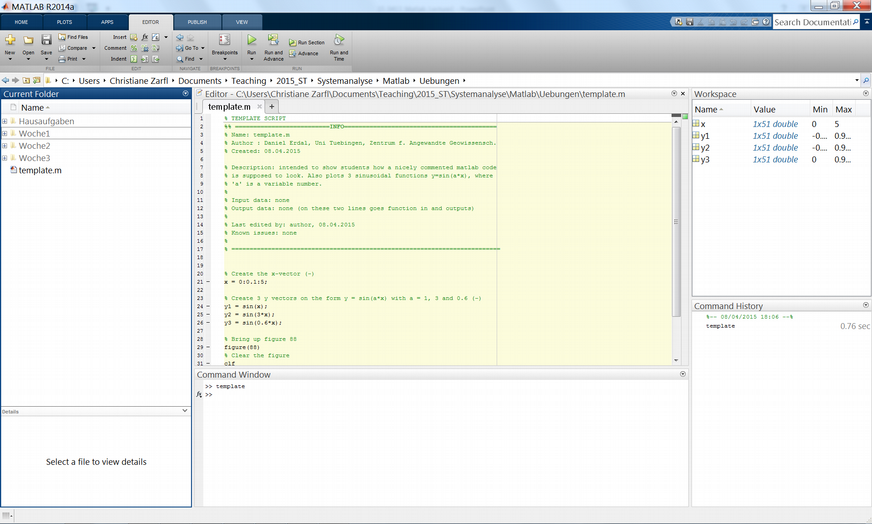
\includegraphics[width=10.0cm]{matlab_gui1.png}};
          \begin{scope}[x={(image.south east)},y={(image.north west)}]
            \node (a) at (0.5, 1.05) {gegenwärtiges Verzeichnis};
            \node[align=left] (b) at (0.1, 0.4) {Dateien im \\gegenwärtigen \\Verzeichnis};
            \node[align=left] (c) at (0.5, 0.5) {Variablen im \\Arbeitsspeicher};
            \node[align=left] (d) at (0.5, 0.15) {Eingabefenster mit \\``Prompt'' (>>)};
            \node[align=left] (e) at (0.85, 0.15) {Eingabe-\\verlauf};
            \draw[line width=0.1cm, ->] (a) -- +(0, -0.2);
            \draw[line width=0.1cm, ->] (b) -- +(0, 0.25);
            \draw[line width=0.1cm, ->] (c) -- +(0.3, 0.15);
            \draw[line width=0.1cm, ->] (e) -- +(0, 0.2);
          \end{scope}
        \end{tikzpicture}
      \end{figure}
    \end{frame}

    \subsection{Hilfe}
    \begin{frame}
      \frametitle{Hilfe in Matlab}
      \begin{itemize}
        \itemsep0.3cm
        \item Niemand kann alle Befehle kennen, deshalb ist die (ausführliche) Hilfe in Matlab so wichtig.
        \item Allgemeines Hilfe-Fenster: \menu{Help > Documentation} (\keys{F1})
        \item Information zu einem Befehl:

        \begin{itemize}
          \itemsep0.3cm
          \item \matlabInput{\matlabLink{doc} <Befehlsname>} (Info in einem extra Fenster)
          \item \matlabInput{\matlabLink{help} <Befehlsname>} (Info im Befehlsfenster)
        \end{itemize}


        \item Beispiele: Im Prompt eingeben:

        \begin{itemize}
          \itemsep0.3cm
          \item \matlabInput{help \matlabLink{sin}}
          \item \matlabInput{help \matlabLink{exp}}
          \item \matlabInput{doc \matlabLink{plot}}
        \end{itemize}
      \end{itemize}
    \end{frame}

    \section{Grundlagen}

    \subsection{Einfaches Rechnen}
    \begin{frame}
      \frametitle{Einfaches Rechnen mit Matlab}
      \begin{itemize}
        \itemsep0.3cm
        \item Alle Anweisungen werden nach dem Prompt (\texttt{>>}) eingegeben und mit \keys{\return} (Return) bestätigt. Matlab nennt das Ergebnis \matlabOutput{ans} (für answer):

        \vspace{-0.3cm}

        \insertMatlabCodeOutput{example1_1}

        \item Addition ($\oplus$), Subtraktion ($\ominus$), Multiplikation ($\otimes$) und Division ($\oslash$) wie im Taschenrechner (Matlab kennt ``Punkt vor Strich-Rechnung'').
        \item Braucht man einen \textbf{Ausdruck öfters}, so kann man ihn als \textbf{Variable} definieren:

        \vspace{-0.3cm}

        \insertMatlabCodeOutput{example1_2}

        \item Variablen werden im Arbeitsspeicher (Workspace) gespeichert (s. Arbeitsspeicher-Fenster).
      \end{itemize}
    \end{frame}

    \begin{frame}
      \frametitle{Grundlegendes}
      \begin{itemize}
        \item Ein Semikolon (;) am Ende der Eingabezeile unterdrückt die Ausgabe des Ergebnisses.
        \item Matlab \textbf{unterscheidet} zwischen Groß- und Kleinbuchstaben!
        \item Potenzieren wird \textbf{vor} einer \textbf{Multiplikation} oder \textbf{Division} ausgewertet, sonst gilt ``Punkt-vor-Strich''; runde Klammern ``('' und ``)'' um die Reihenfolge der Berechnung zu steuern.
        \item Mehrere Anweisungen in einer Zeile sind zulässig:

        \begin{itemize}
          \item Sind sie durch ein Komma getrennt, so folgt eine Ausgabe.
          \item Werden sie durch ein Semikolon getrennt, so folgt keine Ausgabe:

          \vspace{-0.3cm}

          \insertMatlabCodeOutput{example1_3}

        \end{itemize}
      \end{itemize}
    \end{frame}

    \subsection{Variablen}
    \begin{frame}
      \frametitle{Regeln für Variablen}
      \begin{itemize}
        \item Regeln bei der Definition von Variablen:
        \item Das erste Zeichen muss ein Buchstabe sein (Keine Zahl!)
        \item Keine Sonderzeichen (außer Unterstrich)
        \item Max. Zeichenlänge (abhängig vom Computer)
        \item \alert{Vorsicht:} Variablennamen identisch mit Funktionen ist erlaubt, hat aber Seiteneffekte!
        \item Variablen haben einen bestimmten \textbf{Typ}, z.B. Ganzzahl, Fließkommazahl, Vektor, Matrix, ...
      \end{itemize}
    \end{frame}

    \begin{frame}
      \frametitle{Auflisten und Löschen von Variablen}
      \begin{itemize}
        \item \matlabInput{\matlabLink{who}}: gibt eine Liste der Variablen im Arbeitsspeicher aus
        \item \matlabInput{\matlabLink{whos}}: gibt zusätzliche Information (Typ, Größe, Speicherbedarf)
        \item \matlabInput{\matlabLink{clear} <Variable>}: löscht die Variable
        \item \matlabInput{\matlabLink{clear} all}: löscht alle Variablen
        \item \matlabInput{\matlabLink{clc}}: löscht den Inhalt des Befehlsfensters
      \end{itemize}
    \end{frame}

    \secMexercise
    \begin{frame}
      \frameMexercise
      \begin{exercise}
          \sloppy
          Geben Sie nacheinander folgende Anweisungen ein. Überlegen Sie vorher, was Matlab ausgeben wird! \\ \\
          \texttt{u = 2,v = 5;} \keys{\return}\\
          \texttt{(u+6)/4} \keys{\return}\\
          \texttt{y = x+1} \keys{\return}\\
          \texttt{y = 3u} \keys{\return}\\ \\
          Welche der folgenden Variablennamen sind \textbf{nicht} zulässig? \\ \\
          \texttt{anzahl}, \texttt{Summe\_a+b}, \texttt{5\_Tageskarte}, \texttt{dauer\_phase3}, \texttt{sin}
      \end{exercise}
    \end{frame}

    \subsection{Funktionen}
    \begin{frame}
        \frametitle{Einfache Funktionen}
        \begin{itemize}
          \item Es gibt in Matlab bereits ``eingebaute'' Funktionen (viel mehr als im Taschenrechner und Excel).
          \item Z.B. die Wurzelfunktion (square root): \matlabInput{a = \matlabLink{sqrt}(2)/2}
          \item Nähere Informationen zur Funktion \matlabInput{\matlabLink{sqrt}} erhält man mit \matlabInput{help \matlabLink{sqrt}}.
          \item Funktionen können keinen, einen oder mehrere \textbf{Eingabeparameter} haben.
          \item Funktionen können keinen, einen oder mehrere \textbf{Rückgabewerte} haben.
          \item Wie bei Variablen auch haben Funktionen einen bestimmten Typ. D.h. die Ein- und Ausgabewerte \textbf{müssen} vom Typ her passen.
        \end{itemize}
      \end{frame}

      \secMexercise
      \begin{frame}
        \frameMexercise
        \begin{exercise}
            \sloppy
            Berechnen Sie den natürlichen Logarithmus von \texttt{1.36} \\ \\
            Berechnen Sie auch den Logarithmus zur Basis \texttt{10} von \texttt{1.36} \\ \\
            (Zusatz: Wie berechnen Sie den Logarithmus zur Basis \texttt{3} von \texttt{1.36}?)
        \end{exercise}
    \end{frame}

    \secMexercise
    \begin{frame}
      \frameMexercise
      \begin{exercise}
          \sloppy
          Berechnen Sie \texttt{cos($\pi$)} und \texttt{cos($\pi / 2$)} \\ \\
          $\pi$ ist in Matlab bereits eingebaut und wird mit \texttt{pi} bezeichnet \\ \\
          \alert{Vorsicht}: Das Argument der trigonometrischen Funktionen (\texttt{sin, cos, tan, cot}) wird von Matlab immer im \textbf{Bogenmaß} interpretiert \\ \\
          Berechnen Sie den Kosinus von \texttt{180$^{\circ}$} und \texttt{90$^{\circ}$}
      \end{exercise}
    \end{frame}

    \section{Zahlen, Vektoren und Matrizen}

    \subsection{Generelles}
    \begin{frame}
      \frametitle{Zahlen, Vektoren und Matrizen in Matlab}
      \begin{itemize}
          \item Eine Gruppierung von mehreren Zahlenwerten nennt man einen \textbf{Vektor}.
          \item Eine zweidimensionale Gruppierung von Zahlen nennt man eine \textbf{Matrix}.
          \item \textbf{Es folgt}: Eine Zahl ist sowohl ein spezieller Vektor (der Länge \texttt{1}), als auch eine spezielle Matrix der Dimension \texttt{1$\times$1}.
          \item \textbf{Ein Vektor der Länge n} ist eine spezielle Matrix der Dimension \texttt{n$\times$1} (Spaltenvektor) oder \texttt{1$\times$n} (Zeilenvektor).
          \item Matlab (\textbf{MAT}rix \textbf{LAB}oratory) kennt intern nur Matrizen!
          \item Die Berechnung der Wurzel in Matlab von vorhin: \\
          \matlabInput{a = \matlabLink{sqrt}(2)/2} \\
          Hier ist \texttt{a} eine \texttt{1$\times$1} Matrix (selbst die Konstante \texttt{2} wird als eine konstante \texttt{1$\times$1} Matrix interpretiert).
      \end{itemize}
    \end{frame}

    \begin{frame}
      \frametitle{Eingabe von Vektoren}

      \vspace{-0.5cm}

      \begin{itemize}
          \item Vektoren werden in Matlab immer in eckigen Klammern eingegeben: ``['' und ``]''
          \item Die Elemente des Vektors sind durch Leerzeichen (oder ein Komma) zu trennen
          (es ergibt sich ein Zeilenvektor, Semikolon als Trenner ergibt einen Spaltenvektor).
          \item Um in Matlab Tipparbeit zu sparen können Vektoren verwendet werden.
          Möchte man z.B. die Quadratwurzel mehrerer Werte berechnen, so geht man folgendermaßen vor:
          \item Zeilenvektor in einer Variablen definieren: \matlabInput{x = [0 2 4 6 8 10]}.
          \item Die Quadratwurzelfunktion auf den gerade definierten Zeilenvektor \matlabInput{x} anwenden: \matlabInput{y = sqrt(x)}.
          \item Das Ergebnis in der Variablen \matlabInput{y} ist nun ebenfalls ein Zeilenvektor und enthält die einzelnen
          Quadratwurzeln der oben aufgeführten Zahlen.
      \end{itemize}
    \end{frame}

    \begin{frame}
      \frametitle{Elemente von Vektoren}
      \begin{itemize}
          \item Auf die Elemente eines Vektors wird mit der runden Klammer zugegriffen ``()''. Z.B. \matlabInput{x(3)}
          gibt das dritte Element von \matlabInput{x} zurück.
          \item Mit dem Doppelpunkt-Operator \matlabInput{:} (auch \matlabInput{\matlabLink{colon}} genannt) können in Matlab Zahlenfolgen als Vektoren definiert werden. Z.B. kann man
          \matlabInput{x = [0 2 4 6 8 10 12]} kürzer schreiben als \matlabInput{x = 0:2:12}.
          \item Die generelle Syntax lautet: \matlabInput{Startwert:Schrittweite:Endwert} oder \matlabInput{Startwert:Endwert} mit Schrittweite \matlabInput{1}.
          \item Schrittweiten dürfen auch negativ sein: \matlabInput{u = 29:-2:0}
          \item Letztes Element: \matlabInput{x(end)}, vorletztes: \matlabInput{x(end - 1)}
          \item Teile / Bereiche eines Vektors: \matlabInput{x(2:5)}, \matlabInput{x(3:end - 1)}
      \end{itemize}
    \end{frame}

    \secMexercise
    \begin{frame}
      \frameMexercise
      \begin{exercise}
          \sloppy
          Erzeugen Sie einen Vektor \texttt{y}, der die Funktionswerte des natürlichen Logarithmus an den Stellen
          \texttt{x = 1,3,5,7,9} enthält. \\ \\

          Was gibt Matlab aus, wenn Sie \texttt{y(1)} eingeben?
      \end{exercise}
    \end{frame}

    \secMexercise
    \begin{frame}
      \frameMexercise
      \begin{exercise}
          \sloppy
          Geben Sie die Vektoren \texttt{a} und \texttt{b} mit den Elementen
          \texttt{–10,-8,-6,...,6,8,10} bzw. \texttt{10,9,8,...0} mit kurzen Anweisungen ein.
          \alert{Tipp}: \texttt{help colon} \\ \\

          Sei \texttt{x = [1 3 -2 6 0 7 11 -8 -5]}. Finden Sie mit
          \texttt{help paren} und \texttt{help colon} heraus, wie man aus \texttt{x} einen Vektor bildet, der

          \begin{itemize}
              \item das 1., 4. und 9. Element von \texttt{x} enthält
              \item aus den ersten 4 Elementen von \texttt{x} besteht
              \item jedes zweite Element von \texttt{x} enthält.
          \end{itemize}
      \end{exercise}
    \end{frame}

    \subsection{Elementweises Rechnen}
    \begin{frame}
      \frametitle{Elementweises Rechnen mit Vektoren}
      \begin{itemize}
          \item Vektoraddition (-subtraktion) und die Multiplikation (Division) eines Vektors mit einem Skalar sind elementweise definiert durch:
          \item \matlabInput{w = [1 2 3]*2}: Jedes Element des  Vektors \matlabInput{[1 2 3]} wird mit \matlabInput{2} multipliziert und
          in der Variable \matlabInput{w} gespeichert.
          \item \matlabInput{[2 -1 9] + [1 3 6]} ergibt den Vektor \matlabOutput{[3 2 15]}
          \item \alert{Achtung}: Es können nur Vektoren (Matrizen) mit gleichen Dimensionen addiert oder subtrahiert werden!
          \item Die elementweise Addition (Subtraktion) eines Vektors mit einem Skalar ist zulässig, z.B.: \matlabInput{[2 5 7] + 3},
          ergibt \matlabOutput{[5 8 10]}
      \end{itemize}
    \end{frame}

    \begin{frame}
      \frametitle{Elementweises Rechnen mit Vektoren (2)}
      \begin{itemize}
          \item Elementweise Multiplikation, Division und Potenzieren bedarf eines speziellen Operators in Matlab (``Punktoperationen'')
          \item Gegeben seien \matlabInput{a = 1:2:10; b = 1:5;}
          \item Elementweise Multiplikation von a und b: \matlabInput{a.*b}, ergibt hier: \matlabOutput{[1 6 15 28 45]}
          \item Elementweise Division: \matlabInput{a./b}
          \item Elementweises Potenzieren: \matlabInput{a.\string^2}
          \item \alert{Vorsicht}:
          \begin{itemize}
              \item \matlabInput{a} und \matlabInput{b} müssen gleiche Dimension haben!
              \item \matlabInput{a.*b} und \matlabInput{a*b} sind ein großer Unterschied!
          \end{itemize}
      \end{itemize}
    \end{frame}

    \subsection{Multiplikation von Vektoren}

    \begin{frame}
      \frametitle{Multiplikation von Vektoren}
      \begin{itemize}
          \item Der Stern (Asterisk, \matlabInput{*}) in Matlab definiert die übliche Vektormultiplikation.
          \item \matlabInput{a*b} ergibt somit einen Fehler, weil die Dimensionen von \matlabInput{a} und \matlabInput{b}
          \texttt{5$\times$1} ist und diese nicht sinnvoll als Vektoren multipliziert werden können.
          \item Das Apostroph \matlabInput{`} transponiert einen Vektor (oder eine Matrix), \matlabInput{a`} ist also ein Vektor
          der Dimension \texttt{1$\times$5}.
          \item Mit diesem Wissen zurück zur Multiplikation:
          \item \matlabInput{a*b`} ergibt das Skalarprodukt von \matlabInput{a} und \matlabInput{b}.
          \item \matlabInput{a`*b}, ergibt das dyadische Produkt (\texttt{5$\times$5} Matrix).
      \end{itemize}
    \end{frame}

    \secMexercise
    \begin{frame}
      \frameMexercise
      \begin{exercise}
          \sloppy
          Gegeben seien \texttt{a = [1 4 6]} und \texttt{b = [-1 2 1]}.\\ \\

          Was gibt Matlab aus, wenn Sie die folgenden Anweisungen eingeben (geben Sie die Antwort, \textbf{bevor} Sie mit Matlab rechnen!):\\ \\

          \begin{columns}[t]
            \begin{column}{5cm}
                \texttt{a+b} \keys{\return} \\
                \texttt{a*2,a/2} \keys{\return}  \\
                \texttt{a+3} \keys{\return}  \\
                \texttt{a*b} \keys{\return}  \\
            \end{column}

            \begin{column}{5cm}
                \texttt{a.*b} \keys{\return}  \\
                \texttt{a./b} \keys{\return}  \\
                \texttt{a*b`} \keys{\return}  \\
                \texttt{a`*b} \keys{\return}  \\
            \end{column}
          \end{columns}


      \end{exercise}
    \end{frame}

    \secMexercise
    \begin{frame}
      \frameMexercise
      \begin{exercise}
          \sloppy
          Sie möchten einen Vektor \texttt{x} mit den Elementen \texttt{0, 0.2$\pi$, 0.4$\pi$ ...,10$\pi$} definieren.
          Dazu können Sie zum Beispiel die elementweise Multiplikation mit \texttt{$\pi$} verwenden. Welche Möglichkeiten gibt es? \\ \\

          Wie würde Matlab die Anweisung \texttt{y = [0:0.2:10*pi]} interpretieren?
      \end{exercise}
    \end{frame}

    \section{Finally}

    \subsection{Fazit}
    \begin{frame}
      \frametitle{Vorteile und Fallstricke}
      \begin{itemize}
          \item Vorteile:
          \begin{itemize}
              \item Matlab kennt eine große Anzahl an nützlichen Funktionen und Algorithmen (siehe \matlabInput{\matlabLink{doc}})
              \item Rechnen mit Variablen als Platzhaltern ermöglicht einfache Darstellung (Lesbarkeit)
              \item ...
          \end{itemize}
          \item Fallstricke:
          \begin{itemize}
              \item Sequentiell arbeitendes Programm, d.h. Matlab arbeitet Zeile für Zeile.
              \item Eine Variable muss erst definiert werden,
              bevor man sie benutzen kann.
              \item Ändert man den Wert einer Variable, müssen alle Operationen mit dieser Variable wiederholt werden.
              \item Matlab ist ``amerikanisch''
              \begin{itemize}
                  \item Dezimalpunkt statt -komma
                  \item (Standard-)Funktionen haben englische Namen (z.B. ``\matlabInput{\matlabLink{sqrt}}'')
              \end{itemize}
              \item ...
          \end{itemize}
      \end{itemize}
    \end{frame}

    \section{Ausblick}
    \subsection{Ausblick}
    \begin{frame}
      \frametitle{Ausblick}
      \begin{itemize}
          \item Wie kann ich mehrere Rechenschritte/Matlab-Befehle, die ich immer wieder benötige, ``speichern'' und zusammenfassen?
          \item Wie kann ich Ergebnisse von Berechnungen grafisch darstellen?
      \end{itemize}
    \end{frame}

\end{document}
